\input{configTD.tex}

\usepackage{tikz, pgf}
\usetikzlibrary{arrows.meta,patterns,decorations.pathmorphing}
\newcommand{\R}{\mathbb{R}}
\newcommand{\dd}{\mathrm{d}}

\title{Systèmes différentiels et diagonalisation :\\
applications au génie civil}
\author{}
\date{}

\begin{document}
\maketitle

\noindent\textbf{Objectif.}
Utiliser la diagonalisation d'une matrice pour résoudre des systèmes différentiels linéaires couplés issus de problèmes concrets.

\vspace{1.5em}
\hrule
\vspace{1em}

%% ============================================================
%%  EXERCICE 1 — TRANSFERT THERMIQUE (très guidé)
%% ============================================================

\begin{enumerate}[itemsep=2em]

\item \textbf{ Exercice 1 : Transfert thermique entre deux bureaux d'un bâtiment}

\medskip

\begin{center}
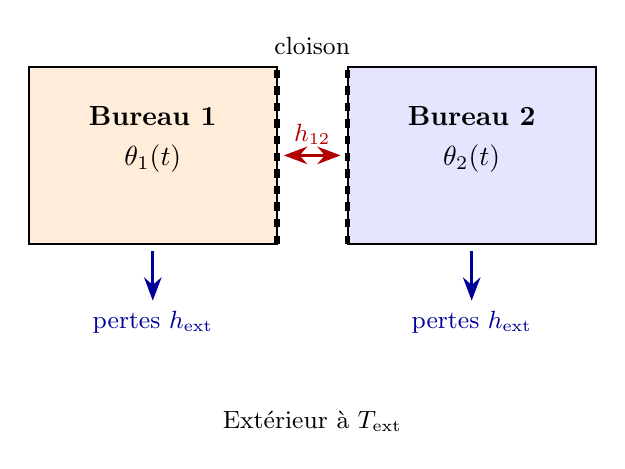
\begin{tikzpicture}[>=Stealth, thick, scale=0.9]
  % Bureau 1
  \draw[fill=orange!15] (0,0) rectangle (3.5,2.5);
  \node at (1.75,1.8) {\textbf{Bureau 1}};
  \node at (1.75,1.2) {$\theta_1(t)$};
  % Bureau 2
  \draw[fill=blue!10] (4.5,0) rectangle (8,2.5);
  \node at (6.25,1.8) {\textbf{Bureau 2}};
  \node at (6.25,1.2) {$\theta_2(t)$};
  % Cloison
  \draw[line width=2pt, dashed] (3.5,0) -- (3.5,2.5);
  \draw[line width=2pt, dashed] (4.5,0) -- (4.5,2.5);
  \node at (4,2.8) {\small cloison};
  % Échanges
  \draw[<->, red!70!black, line width=1.2pt] (3.6,1.25) -- (4.4,1.25)
    node[midway, above, font=\small] {$h_{12}$};
  % Pertes extérieures
  \draw[->, blue!60!black, line width=1.2pt] (1.75,-0.1) -- (1.75,-0.8)
    node[below, font=\small] {pertes $h_{\mathrm{ext}}$};
  \draw[->, blue!60!black, line width=1.2pt] (6.25,-0.1) -- (6.25,-0.8)
    node[below, font=\small] {pertes $h_{\mathrm{ext}}$};
  % Extérieur
  \node at (4,-2.5) {\small Extérieur à $T_{\mathrm{ext}}$};
\end{tikzpicture}
\end{center}

\medskip

Deux bureaux identiques d'un bâtiment sont séparés par une cloison légère. On note $T_{\mathrm{ext}}$ la température extérieure (constante) et on pose :
\[
  \theta_i(t) = T_i(t) - T_{\mathrm{ext}} \qquad (i = 1,2)
\]
l'écart de température de chaque bureau par rapport à l'extérieur. 

La loi de Newton donne que la variation de température $T'$ d'une pièce est proportionnelle à l'écart de température avec l'extérieur multiplié par un coefficient de transfert $h$. 

\medskip

\begin{enumerate}[label=\alph*), itemsep=0.6em]
  \item Écrire les équations de variation de température pour les deux bureaux.

  \item Ecrire le système obtenu sous la forme $X' = AX$ avec $X = \begin{pmatrix} \theta_1 \\ \theta_2 \end{pmatrix}$. Donner explicitement la matrice $A$.

  \item Diagonaliser la matrice $A$, en explicitant la matrice de passage $P$ et la matrice diagonale $D$.

  \item Effectuer le changement d'inconnue $Y = P^{-1}X$, et écrire le nouveau système obtenu avec $Y$.

  \item Résoudre le système d'inconnue $Y$, et en déduire la solution générale du système d'inconnue~$X$.

  \item Le matin, le bureau 1 a été chauffé : $\theta_1(0) = 25\,°\mathrm{C}$, tandis que le bureau 2 est à $\theta_2(0) = 15\,°\mathrm{C}$ au-dessus de l'extérieur. Déterminer les constantes $C_1$ et $C_2$.

  \item Écrire les expressions explicites de $\theta_1(t)$ et $\theta_2(t)$, puis décrire le comportement quand $t \to +\infty$.

  \item \textbf{Interprétation physique des modes propres.}
  \begin{itemize}[nosep]
    \item Le vecteur propre associé à la valeur propre la \emph{plus proche de $0$} : que représente-t-il physiquement ?
    \item Le vecteur propre associé à la valeur propre la \emph{plus négative} : que représente-t-il ?
    \item Quel mode disparaît le plus vite ? Commenter en termes d'isolation de la cloison.
  \end{itemize}
\end{enumerate}

\medskip
\noindent\textbf{Bonus.}
On rallume le chauffage dans le bureau~1 avec une puissance constante : le bilan sur le bureau~1 comporte alors un terme source constant $Q > 0$, soit
\[
  \theta_1' = -3\theta_1 + 2\theta_2 + Q,
\]
les autres équations restant celles obtenues aux questions précédentes.
Le système n'est plus homogène : il s'écrit $X' = AX + B$ avec $B \in \R^2$ constant.

\smallskip
\noindent\textit{Indication.}
À l'équilibre, $AX_{\mathrm{eq}} + B = 0$ ; si $A$ est inversible, alors $X_{\mathrm{eq}} = -A^{-1}B$.
Ensuite, poser $Y = X - X_{\mathrm{eq}}$ : on se ramène à un système homogène en $Y$.

\begin{enumerate}[label=\alph*), itemsep=0.6em]
  \item Que devient le système ? Écrire explicitement le vecteur $B$.
  \item Calculer $X_{\mathrm{eq}}$ à l'aide de $X_{\mathrm{eq}} = -A^{-1}B$.
  \item Effectuer le changement d'inconnue $Y = X - X_{\mathrm{eq}}$ : montrer que $Y' = AY$ et écrire explicitement ce système homogène (de variables $y_1$, $y_2$ si $Y = \begin{pmatrix} y_1 \\ y_2 \end{pmatrix}$).
\end{enumerate}

\vspace{1.5em}
\hrule
\vspace{1em}

\newpage

%% ============================================================
%%  EXERCICE 2 — BASSINS DE RÉTENTION (semi-guidé)
%% ============================================================

\item \textbf{ Exercice 2 : Dépollution de bassins de rétention sur un chantier}

\medskip

Sur un chantier, deux bassins de rétention collectent les eaux de ruissellement chargées en matières en suspension (MES).

\medskip

Les volumes sont $V_A = 200\;\mathrm{m^3}$ pour le bassin~A et $V_B = 100\;\mathrm{m^3}$ pour le bassin~B. Les deux bassins sont reliés par une pompe de recirculation : le débit est $Q = 200\;\mathrm{m^3/h}$ dans chaque sens (échange d'eau entre A et B).

\medskip

En outre, chaque bassin est vidangé vers une station de traitement : le bassin~A au débit $d_A = 400\;\mathrm{m^3/h}$, le bassin~B au débit $d_B = 200\;\mathrm{m^3/h}$. L'eau traitée (propre) est réinjectée de sorte que les volumes $V_A$ et $V_B$ restent constants.

\medskip

On modélise chaque bassin comme un \emph{compartiment à volume constant}. On note $c_1(t)$ et $c_2(t)$ les concentrations en MES dans les bassins A et~B, en~$\mathrm{mg/L}$.

\medskip

Pour un bassin de volume $V$ et de concentration $c(t)$, le \textbf{bilan de masse en polluant} s'écrit
\[
  V\,c'(t) = \underbrace{\text{(flux entrant de polluant)}}_{\text{débit} \times \text{concentration entrante}}
  - \underbrace{\text{(flux sortant de polluant)}}_{\text{débit} \times \text{concentration du bassin}}\,.
\]

\medskip
\begin{enumerate}[label=\alph*), itemsep=0.6em]
  \item En appliquant ce bilan à chaque bassin (recirculation entre A et B, vidanges $d_A$ et $d_B$), montrer que le système s'écrit $X' = AX$ avec $X = \begin{pmatrix} c_1 \\ c_2 \end{pmatrix}$ et
  \[
    A = \begin{pmatrix} -3 & 1 \\ 2 & -4 \end{pmatrix}.
  \]

  \item Diagonaliser $A$ et en déduire la solution générale du système.

  \item En début de journée, les concentrations mesurées sont $c_1(0) = 8\;\mathrm{mg/L}$ et $c_2(0) = 2\;\mathrm{mg/L}$. Déterminer la solution particulière.

  \item La norme impose $c \leq 0{,}5\;\mathrm{mg/L}$ pour rejeter les eaux dans le milieu naturel. Estimer au bout de combien de temps (en heures) les deux bassins respectent cette norme.
\end{enumerate}

\vspace{1.5em}
\hrule
\vspace{1em}

\newpage

%% ============================================================
%%  EXERCICE 3 — OSCILLATIONS SISMIQUES (autonome)
%% ============================================================

\item \textbf{ Exercice 3 : Modes propres de vibration d'un bâtiment à deux étages}

\medskip

\begin{center}
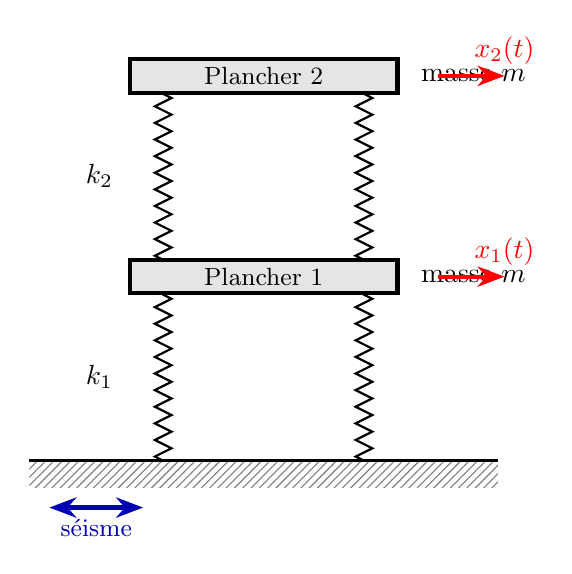
\begin{tikzpicture}[>=Stealth, thick, scale=0.85]
  % Ground
  \fill[pattern=north east lines, pattern color=gray] (-1.5,-0.4) rectangle (5.5,0);
  \draw[very thick] (-1.5,0) -- (5.5,0);
  % Floor 1
  \draw[fill=gray!20, line width=1.5pt] (0,2.5) rectangle (4,3);
  \node[right] at (4.2,2.75) {masse $m$};
  \node at (2,2.75) {\small Plancher 1};
  % Floor 2
  \draw[fill=gray!20, line width=1.5pt] (0,5.5) rectangle (4,6);
  \node[right] at (4.2,5.75) {masse $m$};
  \node at (2,5.75) {\small Plancher 2};
  % Columns ground floor (springs)
  \draw[decorate, decoration={zigzag, segment length=6, amplitude=3}]
    (0.5,0) -- (0.5,2.5);
  \draw[decorate, decoration={zigzag, segment length=6, amplitude=3}]
    (3.5,0) -- (3.5,2.5);
  \node[left] at (-0.1,1.25) {$k_1$};
  % Columns upper floor (springs)
  \draw[decorate, decoration={zigzag, segment length=6, amplitude=3}]
    (0.5,3) -- (0.5,5.5);
  \draw[decorate, decoration={zigzag, segment length=6, amplitude=3}]
    (3.5,3) -- (3.5,5.5);
  \node[left] at (-0.1,4.25) {$k_2$};
  % Displacements
  \draw[->, red, line width=1.5pt] (4.6,2.75) -- (5.6,2.75)
    node[above] {$x_1(t)$};
  \draw[->, red, line width=1.5pt] (4.6,5.75) -- (5.6,5.75)
    node[above] {$x_2(t)$};
  % Seismic arrow
  \draw[<->, blue!70!black, line width=1.5pt] (-1.2,-0.7) -- (0.2,-0.7)
    node[midway, below, font=\small] {séisme};
\end{tikzpicture}
\end{center}

\medskip

On modélise un bâtiment à deux étages par deux masses $m$ (les planchers) reliées par des colonnes modélisées comme des ressorts. On note $x_1(t)$ et $x_2(t)$ les déplacements horizontaux des deux planchers par rapport à leur position d'équilibre.

Les colonnes du rez-de-chaussée ont une raideur totale $k_1 = 300\;\mathrm{kN/m}$, celles de l'étage $k_2 = 200\;\mathrm{kN/m}$. Chaque plancher a une masse $m = 100\;\mathrm{tonnes}$.

\begin{enumerate}[label=\alph*), itemsep=0.6em]
  \item En appliquant le principe fondamental de la dynamique à chaque plancher, établir le système d'équations du mouvement sous la forme $\ddot{X} = -\Omega\, X$, et expliciter la matrice $\Omega$.

  \item Diagonaliser $\Omega$. On notera $\omega_1^2$ et $\omega_2^2$ les valeurs propres.

  \item En déduire les \textbf{pulsations propres} $\omega_1$, $\omega_2$ et les \textbf{périodes propres} $T_1$, $T_2$ du bâtiment.

  \item Décrire physiquement chaque \textbf{mode propre de vibration}. Lequel est le plus dangereux pour la structure et pourquoi ?

  \item Écrire la solution générale $x_1(t)$, $x_2(t)$ comme combinaison des deux modes.
\end{enumerate}

\end{enumerate}

%% ============================================================
%%  CORRIGÉ ENSEIGNANT
%% ============================================================

\makeatletter
\@ifundefined{inclurecorrige}{\end{document}}{}
\makeatother

\newpage
\section*{Éléments de correction (enseignant)}

\paragraph{Exercice 1 — Transfert thermique.}

\textbf{a)} En développant :
\[
\begin{cases}
\theta_1' = -(h_{\mathrm{ext}} + h_{12})\,\theta_1 + h_{12}\,\theta_2 = -3\theta_1 + 2\theta_2, \\[0.3em]
\theta_2' = h_{12}\,\theta_1 - (h_{\mathrm{ext}} + h_{12})\,\theta_2 = 2\theta_1 - 3\theta_2.
\end{cases}
\quad\Longrightarrow\quad
A = \begin{pmatrix} -3 & 2 \\ 2 & -3 \end{pmatrix}.
\]

\textbf{b)} $\chi_A(\lambda) = (\lambda+3)^2 - 4 = \lambda^2 + 6\lambda + 5 = (\lambda+1)(\lambda+5)$.

Valeurs propres : $\lambda_1 = -1$, $\lambda_2 = -5$.

\textbf{c)} Pour $\lambda_1 = -1$ : $(A + I)V = 0 \Rightarrow -2v_1 + 2v_2 = 0$, soit $V_1 = \begin{pmatrix} 1 \\ 1 \end{pmatrix}$.

Pour $\lambda_2 = -5$ : $(A + 5I)V = 0 \Rightarrow 2v_1 + 2v_2 = 0$, soit $V_2 = \begin{pmatrix} 1 \\ -1 \end{pmatrix}$.

\textbf{d)} Solution générale :
\[
  X(t) = C_1\, e^{-t} \begin{pmatrix} 1 \\ 1 \end{pmatrix}
        + C_2\, e^{-5t} \begin{pmatrix} 1 \\ -1 \end{pmatrix}.
\]

\textbf{e)} $X(0) = (25, 15)^\top$ donne $C_1 + C_2 = 25$ et $C_1 - C_2 = 15$, soit $C_1 = 20$, $C_2 = 5$.

\textbf{f)}
\[
  \theta_1(t) = 20\,e^{-t} + 5\,e^{-5t}, \qquad
  \theta_2(t) = 20\,e^{-t} - 5\,e^{-5t}.
\]
Quand $t \to +\infty$, $\theta_1(t) \to 0$ et $\theta_2(t) \to 0$ : les deux bureaux atteignent la température extérieure.

\textbf{g) Interprétation des modes :}
\begin{itemize}[nosep]
  \item \textbf{Mode lent} ($\lambda_1 = -1$, vecteur $(1,1)^\top$) : les deux bureaux refroidissent \emph{ensemble}, à la même vitesse. C'est le mode de refroidissement global vers l'extérieur. Il est lent car seules les façades évacuent la chaleur.
  \item \textbf{Mode rapide} ($\lambda_2 = -5$, vecteur $(1,-1)^\top$) : la \emph{différence} de température entre les deux bureaux s'estompe rapidement. C'est le mode d'équilibrage par la cloison. Il est rapide car la cloison est peu isolante ($h_{12} = 2 \gg h_{\mathrm{ext}} = 1$).
  \item Le mode rapide ($e^{-5t}$) disparaît environ $5\times$ plus vite que le mode lent. En pratique, au bout de $t \approx 0{,}5$~h, les deux bureaux sont déjà quasi à la même température ; le refroidissement global prend bien plus longtemps ($\sim 3$~h). Plus la cloison est isolante (petit $h_{12}$), plus les deux modes ont des constantes de temps proches.
\end{itemize}

\textbf{Bonus.}
\textbf{a)} La deuxième équation est inchangée : $\theta_2' = 2\theta_1 - 3\theta_2$. D'où
$X' = AX + B$ avec $B = \begin{pmatrix} Q \\ 0 \end{pmatrix}$.

\textbf{b)} À l'équilibre, $AX_{\mathrm{eq}} + B = 0$, soit $X_{\mathrm{eq}} = -A^{-1}B$.
On a $\det A = 5$ et
$A^{-1} = \dfrac{1}{5}\begin{pmatrix} -3 & -2 \\ -2 & -3 \end{pmatrix}$, d'où
\[
  X_{\mathrm{eq}}
  = -\frac{1}{5}\begin{pmatrix} -3 & -2 \\ -2 & -3 \end{pmatrix}
    \begin{pmatrix} Q \\ 0 \end{pmatrix}
  = \begin{pmatrix} 3Q/5 \\ 2Q/5 \end{pmatrix}.
\]
Les écarts par rapport à l'extérieur se stabilisent donc à $\theta_{1,\mathrm{eq}} = \dfrac{3Q}{5}$ et $\theta_{2,\mathrm{eq}} = \dfrac{2Q}{5}$ (le bureau~1 reste plus chaud que le bureau~2 car c'est lui qui est chauffé).

\textbf{c)} Avec $Y = X - X_{\mathrm{eq}}$, on a $Y' = X'$ (car $X_{\mathrm{eq}}$ est constant). D'où
$Y' = AX + B = A(Y + X_{\mathrm{eq}}) + B = AY + (AX_{\mathrm{eq}} + B) = AY$.
Le système homogène est donc $Y' = AY$, soit explicitement
\[
\begin{cases}
  y_1' = -3y_1 + 2y_2, \\[0.2em]
  y_2' = 2y_1 - 3y_2,
\end{cases}
\]
le même que pour les écarts $\theta_i$ sans chauffage (on retrouve l'exercice principal, avec des conditions initiales décalées par rapport à $X_{\mathrm{eq}}$).

\bigskip
\paragraph{Exercice 2 — Bassins de rétention.}

\textbf{a)} Bilan de masse sur le bassin~A (volume $V_A = 200$~m$^3$) : entrée de polluant depuis B par la recirculation ($Q\,c_2$), sorties vers B ($Q\,c_1$) et vers la station de traitement ($d_A\,c_1$, l'eau évacuée emporte le polluant à la concentration du bassin).
\[
V_A\, c_1' = \underbrace{Q\, c_2}_{\text{entrée depuis B}}
             - \underbrace{Q\, c_1}_{\text{sortie vers B}}
             - \underbrace{d_A\, c_1}_{\text{vidange vers la station}}.
\]
Soit $c_1' = \dfrac{Q}{V_A}(c_2 - c_1) - \dfrac{d_A}{V_A}\,c_1 = -\dfrac{Q + d_A}{V_A}\,c_1 + \dfrac{Q}{V_A}\,c_2 = -3\,c_1 + c_2$.

De même pour le bassin~B ($V_B = 100$~m$^3$) :
$c_2' = \dfrac{Q}{V_B}\,c_1 - \dfrac{Q + d_B}{V_B}\,c_2 = 2\,c_1 - 4\,c_2$.

D'où $A = \begin{pmatrix} -3 & 1 \\ 2 & -4 \end{pmatrix}$.

\textbf{b)} $\chi_A(\lambda) = (\lambda+3)(\lambda+4) - 2 = \lambda^2 + 7\lambda + 10 = (\lambda+2)(\lambda+5)$.

Valeurs propres : $\lambda_1 = -2$, $\lambda_2 = -5$.

Vecteur propre pour $\lambda_1 = -2$ : $(-3+2)v_1 + v_2 = 0 \Rightarrow V_1 = \begin{pmatrix} 1 \\ 1 \end{pmatrix}$.

Vecteur propre pour $\lambda_2 = -5$ : $(-3+5)v_1 + v_2 = 0 \Rightarrow V_2 = \begin{pmatrix} 1 \\ -2 \end{pmatrix}$.

Solution générale : $X(t) = C_1\, e^{-2t}\begin{pmatrix} 1 \\ 1 \end{pmatrix} + C_2\, e^{-5t} \begin{pmatrix} 1 \\ -2 \end{pmatrix}$.

\textbf{c)} $X(0) = (8, 2)^\top$ donne $C_1 + C_2 = 8$, $C_1 - 2C_2 = 2$, soit $C_1 = 6$, $C_2 = 2$.
\[
  c_1(t) = 6\,e^{-2t} + 2\,e^{-5t}, \qquad
  c_2(t) = 6\,e^{-2t} - 4\,e^{-5t}.
\]

\textbf{d)} Le mode dominant est $6e^{-2t}$. Pour $c_1(t) \leq 0{,}5$ : en négligeant $e^{-5t}$, $6e^{-2t} \approx 0{,}5$ donne $t \approx \frac{1}{2}\ln 12 \approx 1{,}24$~h. Un calcul numérique plus précis (ou une vérification graphique) confirme que les deux bassins satisfont la norme vers $t \approx 1{,}3$~h, soit environ \textbf{1\,h\,15\,min}.

\emph{Remarque} : le bassin~B atteint la norme un peu avant le bassin~A car sa concentration initiale est plus faible et le mode rapide le décontamine en priorité.

\bigskip
\paragraph{Exercice 3 — Oscillations sismiques.}

\textbf{a)} PFD sur le plancher 1 : la force de rappel des colonnes du RDC est $-k_1 x_1$, celle des colonnes de l'étage est $k_2(x_2 - x_1)$. Donc :
\[
m\ddot{x}_1 = -k_1 x_1 + k_2(x_2 - x_1) = -(k_1+k_2)\,x_1 + k_2\, x_2.
\]
PFD sur le plancher 2 : $m\ddot{x}_2 = -k_2(x_2 - x_1) = k_2\,x_1 - k_2\,x_2$.

En divisant par $m = 10^5$~kg et avec $k_1 = 3\times 10^5$~N/m, $k_2 = 2\times 10^5$~N/m :
\[
  \ddot{X} = -\Omega\, X, \qquad
  \Omega = \begin{pmatrix} 5 & -2 \\ -2 & 2 \end{pmatrix} \quad (\text{en s}^{-2}).
\]

\textbf{b)} $\chi_\Omega(\lambda) = (\lambda - 5)(\lambda - 2) - 4 = \lambda^2 - 7\lambda + 6 = (\lambda - 1)(\lambda - 6)$.

Valeurs propres : $\omega_1^2 = 1$, $\omega_2^2 = 6$.

Vecteur propre pour $\omega_1^2 = 1$ : $(5-1)v_1 - 2v_2 = 0 \Rightarrow U_1 = \begin{pmatrix} 1 \\ 2 \end{pmatrix}$.

Vecteur propre pour $\omega_2^2 = 6$ : $(5-6)v_1 - 2v_2 = 0 \Rightarrow U_2 = \begin{pmatrix} 2 \\ -1 \end{pmatrix}$.

\textbf{c)} Pulsations : $\omega_1 = 1\;\mathrm{rad/s}$, $\omega_2 = \sqrt{6} \approx 2{,}45\;\mathrm{rad/s}$.

Périodes : $T_1 = 2\pi \approx 6{,}28\;\mathrm{s}$, $T_2 = 2\pi/\sqrt{6} \approx 2{,}57\;\mathrm{s}$.

\textbf{d) Modes propres :}
\begin{itemize}[nosep]
  \item \textbf{Mode 1} (fondamental, $\omega_1 = 1$~rad/s) : le vecteur $(1,2)^\top$ indique que les deux planchers oscillent \emph{dans le même sens}, le plancher 2 avec une amplitude double. C'est le mode de balancement global, le plus ample et le plus dangereux pour la structure car il sollicite fortement les colonnes du RDC.
  \item \textbf{Mode 2} ($\omega_2 = \sqrt{6}$~rad/s) : le vecteur $(2,-1)^\top$ indique que les planchers oscillent \emph{en sens opposés}. Le plancher 1 a une amplitude double de celle du plancher 2 (en sens inverse). Ce mode sollicite surtout les colonnes de l'étage (cisaillement inter-étage).
\end{itemize}

\textbf{e)} Solution générale : on cherche $X(t) = \phi(t) U$ avec $\ddot{\phi} = -\omega^2 \phi$, soit $\phi(t) = A\cos(\omega t + \varphi)$.
\[
\begin{pmatrix} x_1(t) \\ x_2(t) \end{pmatrix}
= A_1 \cos(\omega_1 t + \varphi_1) \begin{pmatrix} 1 \\ 2 \end{pmatrix}
+ A_2 \cos(\omega_2 t + \varphi_2) \begin{pmatrix} 2 \\ -1 \end{pmatrix},
\]
soit :
\[
  x_1(t) = A_1\cos(t + \varphi_1) + 2A_2\cos(\sqrt{6}\,t + \varphi_2),
\]
\[
  x_2(t) = 2A_1\cos(t + \varphi_1) - A_2\cos(\sqrt{6}\,t + \varphi_2).
\]
Les quatre constantes $A_1, A_2, \varphi_1, \varphi_2$ sont déterminées par les positions et vitesses initiales.

\end{document}
